
\section{Rigid区域处理}

对采集到的图像进行直方图统计分析, 发现Rigid区域的典型特征就是像素占比高且灰度值低, 在15以内(见图.\ref{fig:hist}),  所以通过设置灰度值门限的方法能一定程度上对其分类, 即
\begin{figure}[t]
	\begin{center}
		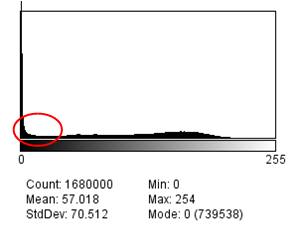
\includegraphics[width=0.75\linewidth]{src/hist}
	\end{center}
	\caption{典型的原图像的灰度直方图统计,可见在门限值约为20以内的像素占绝大多数(红圈标注).}
	\label{fig:hist}	
\end{figure}
\begin{eqnarray}
	\quad M_r(p) = [I(p) \le \delta_r ]
\end{eqnarray}


但通过此类方法会将其他区域一些低灰度点误判为Rigid 区域, 所以这里引入图像形态学方法\cite{GonzalezW08}对此类区域进行矫正处理.
\begin{figure}[t]
	\begin{center}
		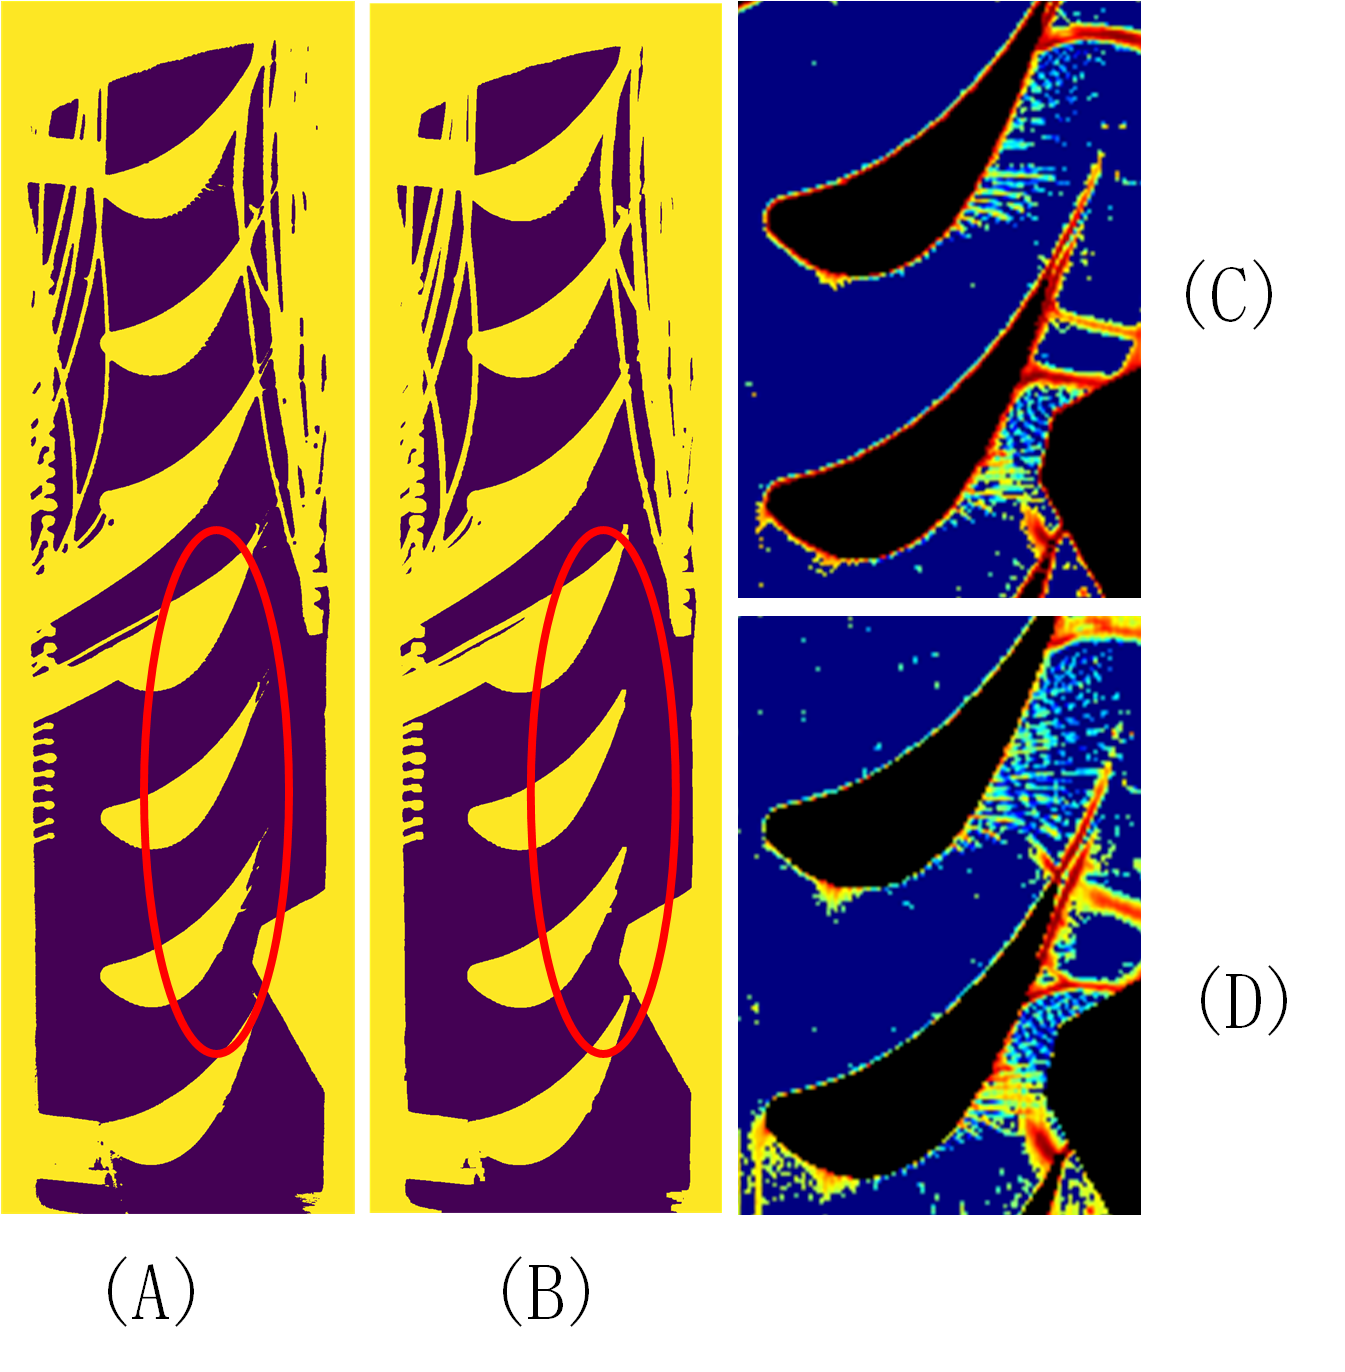
\includegraphics[width=0.75\linewidth]{src/rigid}
	\end{center}
	\caption{(A)(B)分别为$M_r$膨胀腐蚀操作前与操作后,(C)(D)分别为经过处理前与处理后的不同结果. 可以看到膨胀腐蚀操作去除了孤立点(红色圈出), 并且能有效改善叶片边缘处像素分类为Flow区域并带入渲染造成的红圈错误.}
	\label{fig:rigid}	
\end{figure}

具体来讲, 通过图像腐蚀, 能将二值图像$M_r(p)$的孤立点进行抹除, 但同时也会对边缘部分进行消去,带来的影响就是结果在叶片边缘区域会有红色条纹, 所以我们在腐蚀操作后, 对其进行膨胀操作, 使得整体而言, 在消除孤立点的同时不损失边缘, 减少叶片边缘处的红线(图.\ref{fig:rigid}).

对不同的数据集, 光线的明暗也许会对$\delta_r$的选择带来影响, 为了选择更好的$\delta_r$, 在数据量充足的情况下应对整个图像进行直方图统计, 使得能够自动的设置合适的门限值.